\documentclass[12pt, a4paper]{article}

\usepackage[utf8]{inputenc}
\usepackage[brazil]{babel}
\usepackage[left=2cm, right=2cm, top=2cm, bottom=2cm]{geometry}
\usepackage{hyperref}
\usepackage{setspace}
\usepackage{graphicx}
\usepackage{mathtools}
\usepackage{amsmath}
\usepackage{color}

\bibliographystyle{plain}

\setlength{\parskip}{6pt}
\setlength{\parindent}{1.5cm}

\hypersetup{
   colorlinks,
   linkcolor={red},
   citecolor={blue}, 
   urlcolor={blue},
   pdfsubject={Ramanujan},
   pdfauthor={Carla Negri Lintzmayer},
   pdftitle={Um breve relato sobre Ramanujan}
}

\onehalfspacing

\author{Thiago F. Dias}
\title{\textbf{\underline{Um breve relato sobre Ramanujan}}}

\thispagestyle{empty}

\date{\today}

\begin{document}

\begin{center}
    \textsc{\bf Universidade Federal do ABC}\\
    \textsc{IV Semana do CMCC -- \today}\\[0.2cm]
    
    \hrulefill 

    \textbf{\large \underline{Um breve relato sobre Ramanujan}}
    
    \textsc{\small (Minicurso Introdução ao \LaTeX)}
    
    \hrulefill
    \vspace{0.5cm}
    
    \begin{minipage}{0.4\textwidth}
    \begin{flushleft}
    \emph{Autor:}\\
    Thiago F. Dias
    \end{flushleft}
    \end{minipage}
    \begin{minipage}{0.5\textwidth}
    \begin{flushright}
    \emph{Instrutora:} \\
    Carla Negri Lintzmayer
    \end{flushright}
    \end{minipage}
\end{center}

\begin{abstract}
\indent 
Um misterioso matemático, nascido em 1887 em Erode, na Índia, criou
teoremas surpreendentes. Sem formação acadêmica, realizou contribuições
substanciais nas áreas da análise matemática, teoria dos números, séries
infinitas, frações continuadas, \ldots Esse documento conta um pouco de 
sua história.
\end{abstract}

{\singlespacing\setlength{\parskip}{0pt} \listoffigures}
{\singlespacing\setlength{\parskip}{0pt} \listoftables}
{\singlespacing\setlength{\parskip}{0pt} \tableofcontents}

\newpage

\section{Introdução}\label{sec:intro}
\noindent 
Srinivasa Aiyangar Ramanujan (Erode, 22 de dezembro de 1887 -- Kumbakonam, 26 
de abril de 1920), foi um matemático indiano.  Seus estudos nunca foram 
efetivamente publicados.  O que existe da sua obra são essencialmente fórmulas 
e expressões matemáticas isoladas e rascunhos manuscritos.

Ramanujan era um matemático com um modo de trabalhar especial.  Embora não
tivesse o conceito de demonstração enraizado, a verdade é que possuía uma
intuição admirável.  São muitas as contribuições do matemático, sendo ele
considerado um gênio marcante para os estudos das ciências exatas.

Ao procurar por matemáticos que pudessem entender seu trabalho, em 1913 ele
começou a trocar cartas com G. H. Hardy\footnote{Godfrey Harold Hardy foi um 
matemático inglês, conhecido por seu trabalho em teoria dos números e análise 
matemática.} da Universidade de Cambridge, Inglaterra.  Eventualmente Hardy 
trouxe Ramanujan para o Trinity College de
Cambridge, onde os dois deram início a uma frutuosa relação de trabalho.

Com saúde muito frágil por vários anos, ele morreu em 1920, em Kumbakonam, na
Índia.  Sua história é relatada no filme intitulado \textit{The Man Who Knew 
Infinity} (''O homem que viu o infinito'')
\marginpar{\footnotesize Esse filme teve orçamento de \$10 milhões.}, de 2015, 
que por sua vez é baseado em um livro de 1991, de mesmo nome.

O restante desse documento está dividido da seguinte forma. Na
Seção~\ref{sec:vida} apresentamos alguns dos eventos mais importantes sobre a 
vida de Ramanujan. Na Seção~\ref{sec:resultados} apresentamos alguns dos 
resultados obtidos pelo matemático. Na Seção~\ref{sec:cultura_popular} mostramos 
como a história do Ramanujan já foi inserida na cultura popular. Por fim, na 
Seção~\ref{sec:publicacoes} indicamos algumas de suas publicações.

\section{Vida}\label{sec:vida}

\noindent 
Srinivasa Ramanujan tem uma história de vida bastante interessante e cheia de
detalhes. A seguir tentamos resumir os eventos mais importantes:

\begin{description}
    \item[1887] Nasceu em Erode, Tamil Nadu, India, em 22 de dezembro;
    \begin{itemize}
        \item Filho de K. Srinivasa Iyengar \& Komalatammal.
    \end{itemize}
    \item[1906] Entrou na Universidade Pachaiyappa, em Madras, mas saiu sem 
                completar os estudos;
    \item[1911] Publicou primeiro artigo sobre Números de Bernoulli;
    \item[1913] Escreve a primeira carta a G. H. Hardy;
    \item[1914] E. H. Neville conhece Ramanujan em Madras e o convence a ir para 
                Cambridge;
    \item[1916] Consegue grau de bacharel na Universidade de Cambridge;
    \item[1917] É constantemente hospitalizado para tratamentos;
    \item[1918] Se torna \textit{Fellow of the Royal Society};
    \item[1919] Eleito para bolsa de estudos no Trinity College em Cambridge;
    \item[1920] De volta à Índia, com piora na saúde, morre em 26 de Abril de
                1920.
\end{description}

\begin{figure}[h!]
\caption{Ramanujan}\label{fig:ramanujan}
\centering
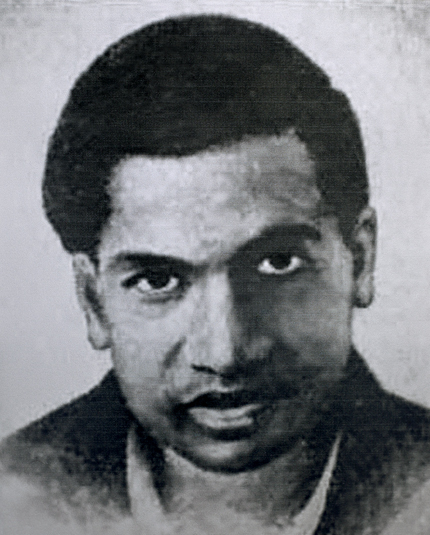
\includegraphics[scale=2.5]{ramanujan.png}
\end{figure}

Veja na Figura~\ref{fig:ramanujan} uma foto de Ramanujan. 

\section{Resultados notáveis}\label{sec:resultados}
\noindent
Ramanujan é bastante conhecido por resultados como
\begin{itemize}
    \item Constante de Landau-Ramanujan
    \item Função teta de Mock
    \item Primo Ramanujan
    \item Constante de Ramanujan-Soldner
    \item Função teta de Ramanujan
    \item Soma de Ramanujan
    \item Identidades de Rogers-Ramananujan
\end{itemize}

Em matemática, há uma distinção entre ter uma introspecção e ter uma prova. O 
talento de Ramanujan sugeriu uma infinidade de fórmulas que somente poderiam ser
investigadas em profundidade mais tarde. Como um subproduto, novas linhas de
investigação se abriram. Exemplos do mais interessante destas fórmulas inclui a
série infinita intrigante para $\pi$, que é dada na
Equação~\eqref{eq:serie_infinita_para_pi} a seguir.

\begin{equation}\label{eq:serie_infinita_para_pi}
   \frac{1}{\pi} = \frac{2\sqrt{2}}{9801} \sum_{k=0}^\infty
   \frac{(4k)!(1103+26390k)}{(k!){^4} 396^{4k}}
\end{equation}

Em 1919, Ramanujan publicou uma nova prova para o postulado de Bertrand e, ao
fim da prova, derivou um resultado mais geral, que é

\noindent
$ \pi(x) - \pi\left(\frac{x}{2}\right) \geq 1,2,3,4,5,\ldots $ para todo
$ x \geq 2,11,17,29,41,\ldots $ respectivamente, onde $ \pi(x) $ é o número de
primos menores ou iguais a x.

O inverso desse resultado é a definição de primos de Ramanujan. O $n$-ésimo
primo de Ramanujan é o menor inteiro $ R_{n} $ para o qual 
$ \pi(x) - \pi\left(\frac{x}{2}\right) \geq n $, para todo $ R_{n} \leq x $.

\subsection{Quadrado Mágico}\label{subsec:quadrado_magico}
\noindent
Uma matriz quadrada de inteiros é um Quadrado Mágico se a soma dos elementos de
cada linha, a soma dos elementos de cada coluna, a soma dos elementos da 
diagonal principal e da diagonal secundária são todos iguais.

\begin{center}
    \begin{tabular}{|c|c|c|c|}
        \hline
        22 & 12 & 18 & 87 \\ \hline
        88 & 17 & 9 & 25 \\ \hline
        10 & 24 & 89 & 16 \\ \hline
        19 & 86 & 23 & 23 \\ \hline
    \end{tabular}
\end{center}

\subsection{O número 1729}

\noindent
O número 1729 ficou conhecido como número de Hardy-Ramanujan após uma visita que
Hardy fez a Ramanujan no hospital:

\begin{quote}
-Hardy, qual o número do taxi que você veio?\\
-Um número sem importância, sem relevância, era o 1729.\\
-Não Hardy, esse é um belo número. Ele é o menor inteiro formado pela soma de 
 dois outros inteiros elevados ao cubo!
\end{quote}

As duas formas são $ 1729 = 10^3 + 9^3 = 1^3 + 12^3 $.

Generalizações dessa ideia criaram a noção de números taxicab.

\section{Na cultura popular}\label{sec:cultura_popular}

\noindent
A Tabela~\ref{table:na_cultura_popular} apresenta algumas informações sobre
aparições da história de Ramanujan na cultura popular~\cite{wikipedia}.

\begin{table}[h!]
    \caption{Ramanujan na cultura popular}\label{table:na_cultura_popular}
    \centering
    \begin{tabular}{c||p{0.4\textwidth}|p{0.4\textwidth}}
        \textbf{ Ano } & \textbf{ O que? } & \textbf{ Detalhes } \\ \hline
        1988 & documentário \textit{The Man Who Loved Numbers} & Série NOVA da
        PBS \\ \hline
        1991 & livro \textit{The Man Who Knew Infinity: A Life of the Genius
        Ramanujan} & biografia escrita por Robert Kanigel \\ \hline
        1006 & peça \textit{First class man} & centrada na relação entre
        Ramanujan e Hardy \\ \hline
        2015 & filme \textit{The Man Who Knew Infinity} & Dev Patel interpretou
        Ramanujan \\ \hline
    \end{tabular}
\end{table}

\section{Publicações}\label{sec:publicacoes}

\noindent
Um dos artigos em conjunto de Ramanujan e Hardy foi publicado em 
1917~\cite{1917-hardy-ramanujan}.

Ramanujan publicou 37 artigos que, após a sua morte, foram reunidos em um
livro~\cite{2000-aiyangar-etal}.

\addcontentsline{toc}{section}{Referências Bibliográficas}
\bibliography{Bibliografia}

\end{document}
